% TODO: discuss more related works: sparsity, and actual implementations.
% TODO: Explain why we are using Stanford
\documentclass[preprint]{elsarticle}

% Packages that I must import to compile this latex file:
\usepackage{amssymb}    % To use \mathbb
\usepackage{amsmath}    % To use the equation environment
\usepackage{graphicx}   % For includegraphics
\usepackage{mathpartir} % To use \inferrule

\newcommand\BibTeX{{\rmfamily B\kern-.05em \textsc{i\kern-.025em b}\kern-.08em
T\kern-.1667em\lower.7ex\hbox{E}\kern-.125emX}}

\def\volumeyear{2012}

% New environments that I use to organize the text:
\newtheorem{definition}[section]{Definition}

% Definition of new commands that I use in this text:
\newcommand{\fun}[1]{\mbox{\textbf{#1}}}
\newcommand{\lb}[1]{#1_{\downarrow}}
\newcommand{\ub}[1]{#1_{\uparrow}}
\newcommand{\varset}[1]{\mbox{$\cal{#1}$}}

\journal{Computer Languages, Systems and Structures}

\begin{document}

\begin{frontmatter}

\title{Speed and Precision in Range Analysis}

%\author{Victor Hugo Sperle Campos, Douglas do Couto Teixeira \\
%Igor Rafael Assis Costa, Raphael Ernani Rodrigues and\\
%Fernando Magno Quint\~{a}o Pereira%\corrauth
%}

\author[llp]{Victor Hugo Sperle Campos}
\ead{victorsc@dcc.ufmg.br}

\author[llp]{Douglas do Couto Teixeira}
\ead{douglas@dcc.ufmg.br}

\author[llp]{Igor Rafael de Assis Costa}
\ead{igor@dcc.ufmg.br}

\author[llp]{Raphael Ernani Rodrigues}
\ead{raphael@dcc.ufmg.br}

\author[llp]{Fernando Magno Quint\~{a}o Pereira\corref{cor1}}
\ead{fernando@dcc.ufmg.br}

\cortext[cor1]{Corresponding author}

\address[llp]{UFMG -- 6627 Ant\^{o}nio Carlos Av, 31.270-010, Belo Horizonte, Brazil}

\begin{abstract}
Range analysis estimates statically the lower and upper values that
the variables may assume during a program's execution.
This analysis is used to detect program vulnerabilities, and to enable compiler
optimizations such as dead and redundant code elimination.
This paper describes an inter-procedural range analysis of integer variables
that scales up to programs with millions of assembly instructions.
Contrary to previous techniques, we handle comparisons between variables
without resorting to relational lattices or expensive algorithms.
We gain precision from conditional tests by using Bodik's Extended Static
Single Assignment intermediate representation, and we obtain partial
context sensitiveness via function inlining.
We have implemented our technique in LLVM and have been able to process
programs totaling 2.72 million lines of C in a few seconds.
During the effort to produce an industrial-quality implementation of our
algorithm, we had to face a constant tension between precision and speed.
In this paper we discuss the many engineering choices that, due to this tension,
have shaped our implementation.
Given the breath of our evaluation, we believe that this paper contains the most
comprehensive empirical study of a range analysis algorithm ever presented in
the compiler related literature.
\end{abstract}

\begin{keyword}
kw1 \sep kw2 \sep kw3
\end{keyword}

\end{frontmatter}

\section{Introduction}

% The context: why range analysis is necessary.
The analysis of integer variables on the interval lattice has been the
canonical example of abstract interpretation since its introduction in
Cousot and Cousot's seminal paper~\cite{Cousot77}.
Compilers use range analysis to infer the possible values that discrete
variables may assume during program execution.
This analysis has many uses.
For instance, it allows the optimizing compiler to remove from the program text
redundant overflow tests~\cite{Sol11} and unnecessary array bound
checks~\cite{Bodik00,Gampe11}.
Furthermore, range analysis is essential to bitwidth aware register
allocators~\cite{Barik06,Tallam03}, register allocators that handle registers of
different sizes~\cite{Kong98,Pereira08,Scholz02}, and scratchpad cache
allocators~\cite{Yanqin11}.
Additionally, range analysis has also been used to statically predict the
outcome of branches~\cite{Patterson95}, to detect buffer overflow
vulnerabilities~\cite{Simon08,Wagner00}, to find the trip count of
loops~\cite{Lokuciejewski09}
and even to synthesize hardware~\cite{Cong05,Lhairech10,Mahlke01}.

% The problem: few implementations, not extensive experimental reports.
Given this great importance, it comes as no surprise that the compiler
literature is rich in works describing in details algorithmic variations of
range analyses~\cite{Mahlke01,Gawlitza09,Stephenson00,Su05}.
On the other hand, none of these authors provide experimental evidence that
their approaches are able to deal with very large programs.
There are researchers who have implemented range analyses that scale up to
large programs~\cite{Patterson95,Blanchet03,Venet04}; nevertheless, because the
algorithm itself is not the main focus of their works, they neither give
details about their design choices nor provide experimental data about it.
This scenario was recently changed by Oh {\em et al.}~\cite{Oh12}, who
introduced an abstract interpretation framework which processes programs with
hundreds of thousands of lines of code.
Nevertheless, Oh {\em et al.} have designed a simple range analysis,
which does not handle comparisons between variables, for instance.
They do not discuss the precision of their implementation, but only its
runtime and memory consumption.
In this paper we claim to push this discussion considerably further.

% Our contribution.
In this paper we provide a complete description of a range analysis algorithm,
and show extensive experimental data that justifies our engineering choices.
Our first algorithmic contribution on top of previous works is a three-phases
approach to handle comparisons between variables without resorting to any
exponential time technique.
The few publicly available implementations of range analyses that we are
aware of, such as those in FLEX~\footnote{The MIT's FLEX/Harpoon compiler
provides an implementation of Stephenson's algorithm~\cite{Stephenson00}, and
is available at \texttt{http://flex.cscott.net/Harpoon/}.},
gcc~\footnote{Gcc's VRP pass (at \texttt{http://gcc.gnu.org/svn/gcc/trunk/gcc/tree-vrp.c}) implements a variant of Patterson's
algorithm~\cite{Patterson95}.} or Mozilla's IonMonkey~\footnote{\texttt{hg.mozilla.org/projects/ionmonkey/file/629d1e6251b9/js/src/ion/RangeAnalysis.cpp}} only deal with comparisons between variables and
constants.
Even theoretical works, such as Su and Wagner's~\cite{Su05} or Gawlitza
{\em et al.}'s~\cite{Gawlitza09} suffer from this limitation.
This deficiency is one of the reasons explaining why none of these works has
made their way into industrial-strength compilers.
Two other insights allow our implementation to scale up to very large
programs.
We use Bodik's Extended Static Single Assignment (e-SSA) form~\cite{Bodik00} to
perform path-sensitive range analysis sparsely.
This program representation ensures that the interval associated with
a variable is constant along its entire live range.
Finally, we process the strongly connected components that underline our
constraint system in topological order.
It is well-known that this technique is essential to speedup constraint solving
algorithms~\cite[Sec 6.3]{Nielson99}; however, due to our three-phases
approach, a careful propagation of information along strong components not only
gives us speed, but also improves the precision of our results.

% Our experimental numbers.
We have implemented our algorithm in the LLVM compiler~\cite{Lattner04}, and
have used it to process a test suite with 2.72 million lines of C code.
As we show in Section~\ref{sub:showdown}, our implementation, which is
publicly available, is able to analyze programs with over one million assembly
instructions within fifteen seconds.
And our implementation is not a straw-man: it produces very precise results.
We have compared the ranges that our implementation finds with the results
obtained via a dynamic profiler, which we have also implemented.
As we show in Section~\ref{sub:showdown}, when analyzing well-known numeric
benchmarks we are able to estimate tight ranges for almost half of all the
integer variables present in these programs.
Our results are similar to Stephenson
{\em et al}'s~\cite{Stephenson00}, even though our analysis does not require
a backward propagation phase.
Furthermore, we have been able to find tight bounds to the majority of the
examples used by Costan {\em et al.}~\cite{Costan05} and Lakhdar
{\em et al.}~\cite{Lakhdar11}, who rely on more costly methods.

% Design space exploration:
While designing and implementing our algorithm we had to face several important
engineering decisions.
Many approaches that we have used to increase the precision of
our results would result in runtime slowdowns.
We cannot determine the optimum spot in this design space, given the
vast number of possibilities that it contains, but we discuss our most important
implementation choices in Section~\ref{sec:design}.
Section~\ref{sub:sccs} shows how we could improve runtime and precision
substantially by processing data-flow information in the strongly connected
components that underly our constraint system.
Section~\ref{sub:program_rep} discuss the importance of choosing a suitable
intermediate representation when implementing a sparse data-flow framework.
Section~\ref{sub:whole} compares the intra-procedural and the inter-procedural
versions of our algorithm.
The role of context sensitiveness is discussed in Section~\ref{sub:context}.
Finally, Section~\ref{sub:widen} discusses the different widening strategies
that we have experimented with.

% The history of our contribution.
This work concludes a two years long effort to produce a solid and scalable
implementation of range analysis.
Our first endeavor to implement such an algorithm was based on Su and
Wagner's constraint system, which can be solved exactly in polynomial
time~\cite{Su05,Su04}.
However, although we could use their formulation to handle a subset of C-like
constructs, their description of how to deal with loops was not very explicit.
Thus, in order to solve loops we adopted Gawlitza
{\em et al.}'s~\cite{Gawlitza09} approach.
This technique uses the Bellman-Ford algorithm to detect increasing or
decreasing cycles in the constraint system, and then saturates these cycles
via a simple widening operator.
A detailed description of our implementation has been published by
Couto and Pereira~\cite{Couto11}.
Nevertheless, the inability to handle comparisons between variables, and the
cubic complexity of the Bellman-Ford method eventually led us to seek
alternative solutions to range analysis.
This quest reached a pinnacle in the present work.

\section{Background}
\label{sec:bck}

% Define the lattice, the constraints and the valuation I.
Following Gawlitza {\em et al.}'s notation, we shall be performing arithmetic
operations over the complete lattice
$\cal{Z} = \mathbb{Z} \cup \{-\infty, +\infty\}$, where the ordering is
naturally given by $-\infty < \ldots < -2 < -1 < 0 < 1 < 2 < \ldots +\infty$.
For any $x > -\infty$ we define:

\begin{tabular}{lcl}
$x + \infty = \infty, x \neq -\infty$ & \mbox{\hspace{0.1cm}} & $x - \infty = - \infty, x \neq +\infty$ \\
$x \times \infty = \infty$ if $x > 0$ & & $x \times \infty = -\infty$ if $x < 0$ \\
$0 \times \infty = 0$ & & $(-\infty) \times \infty = \ $ not defined $$ \\
\end{tabular}

From the lattice $\varset{Z}$ we define the product lattice
$\varset{Z}^2$, which is defined as follows:
%
\begin{equation*}
\varset{Z}^2 = \{ \emptyset \} \cup \{[z_1, z_2] | \ z_1,z_2 \in \varset{Z},
\ z_1 \leq z_2, \  -\infty < z_2 \}
\end{equation*}
%
This interval lattice is partially ordered by the subset relation, which we
denote by ``$\sqsubseteq$".
The meet operator ``$\sqcap$" is defined by:
\[
[a_1, a_2] \sqcap [b_1, b_2] =
\begin{cases}
[\mbox{max}(a_1, b_1), \mbox{min}(a_2, b_2)], \ \mbox{if} \ a_1 \leq b_1 \leq a_2 \ \mbox{or} \ b_1 \leq a_1 \leq b_2 \\
[a_1, a_2] \sqcap [b_1, b_2] = \emptyset, \ \mbox{otherwise}
\end{cases}
\]


Given an interval $\iota = [l, u]$, we let $\lb{\iota} = l$, and
$\ub{\iota} = u$.
We let \varset{V} be a set of constraint variables, and
$I: \varset{V} \mapsto \varset{Z}^2$ a
mapping from these variables to intervals in $\varset{Z}^2$.
Our objective is to solve a constraint system $C$, formed by constraints such
as those seen in Figure~\ref{fig:eval_function}(left).
We let the $\phi$-functions be as defined by Cytron
{\em et al.}~\cite{Cytron91}: they join different variable names into a single
definition.
Figure~\ref{fig:eval_function}(right) defines a valuation function $e$ on the
interval domain.
Armed with these concepts, we define the range analysis problem as follows:

\begin{definition}
\label{def:rcp}
\textsc{Range Analysis Problem} \\
\textbf{Input:} a set $C$ of constraints ranging over a set \varset{V} of
variables. \\
\textbf{Output:} a mapping I such that, for any variable
$V \in \varset{V}$, e(V) = I[V].
\end{definition}

\begin{figure}[t!]
\begin{center}
\begin{small}
\begin{eqnarray*}
\begin{array}{r@{\hspace{1.5cm}}c}
Y = [l, u]
&
e(Y) = [l, u]
\\
\\
Y = \phi (X_1, X_2)
&
\inferrule{I[X_1]=[l_1, u_1] \\ I[X_2]=[l_2, u_2]}
{e(Y) = [\mbox{min}(l_1, l_2), \mbox{max}(u_1, u_2)]}
\\
\\
Y = X_1 + X_2
&
\inferrule{I[X_1]=[l_1, u_1] \\ I[X_2]=[l_2, u_2]}
{e(Y) = [l_1 + l_2, u_1 + u_2]}
\\
\\
Y = X_1 \times X_2
&
\inferrule{I[X_1]=[l_1, u_1] \\ I[X_2]=[l_2, u_2] \\ L = \{l_1l_2, l_1u_2, u_1l_2, u_1u_2\}}
{e(Y) = [\mbox{min}(L), \mbox{max}(L)]}
\\
\\
Y = aX + b
&
\inferrule{I[X]=[l, u] \\ k_l = al + b \\ k_u = au + b}
{e(Y) = [\mbox{min}(k_l, k_u), \mbox{max}(k_l, k_u)]}
\\
\\
Y = X \sqcap [l', u']
&
\inferrule{I[X]=[l, u]}
{e(Y) \leftarrow [\mbox{max}(l, l'), \mbox{min}(u, u')]}
\end{array}
\end{eqnarray*}
\caption{\label{fig:eval_function}
A suite of constraints that produce an instance of the range analysis problem.}
\end{small}
\end{center}
\end{figure}

We will use the program in Figure~\ref{fig:ex1}(a) as the running example
to illustrate our range analysis.
Figure~\ref{fig:ex1}(b) shows the same program in SSA form~\cite{Cytron91},
and Figure~\ref{fig:ex1}(c) outlines the constraints that we extract from this
program.
There is a clear correspondence between instructions and constraints.
A possible solution to the range analysis problem, as obtained via the
techniques that we will introduce in Section~\ref{sec:algo}, is given in
Figure~\ref{fig:ex1}(d).
The SSA form, so common in modern compilers, leads to a very conservative
solution.
As we will see shortly, we can improve this solution substantially by using
a more sophisticated program representation -- the e-SSA form -- which
gives us path-sensitiveness.

\begin{figure}[t!]
\begin{center}
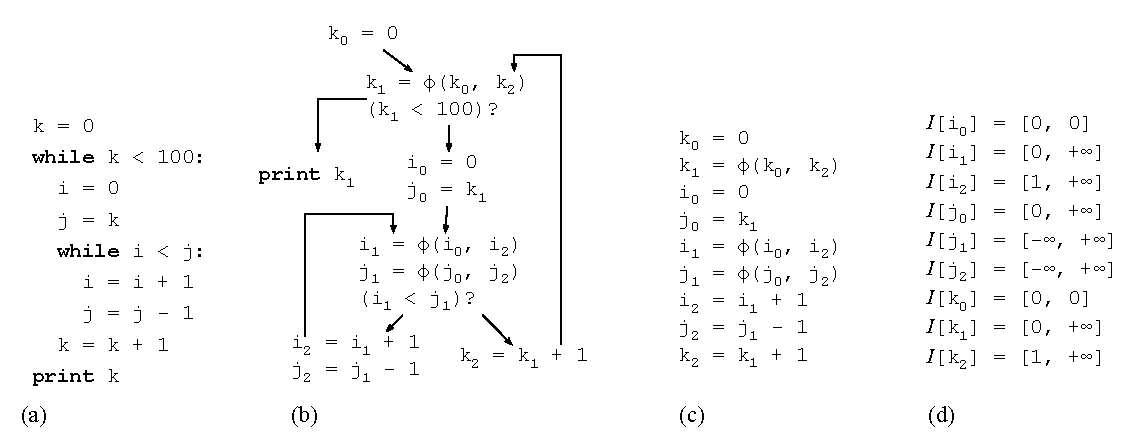
\includegraphics[width=1\textwidth]{images/ex1}
\end{center}
\caption{\label{fig:ex1}
(a) Example program.
(b) Control Flow Graph in SSA form.
(c) Constraints that we extract from the program.
(d) Possible solution to the range analysis problem.}
\end{figure}

\section{Our Design of a Range Analysis Algorithm}
\label{sec:algo}

% Program representation
% Extracting constraints
% Building the Constraint graph (pseudo-edges)
% Macro algorithm
% Micro algorithm

In this section we explain the algorithm that we use to solve the range
analysis problem.
This algorithm involves a number of steps.
First, we convert the program to a suitable intermediate representation that
makes it easier to extract constraints.
From these constraints, we build a dependence graph that allows us to do
range analysis sparsely.
Finally, we solve the constraints applying different fix-point iterators on
this dependence graph.
Figure~\ref{fig:algorithm} gives a global view of this algorithm.
Some of the steps in the algorithm are optional.
They improve the precision of the range analysis, at the expense of a longer
running time.

\begin{figure}[t!]
\begin{center}
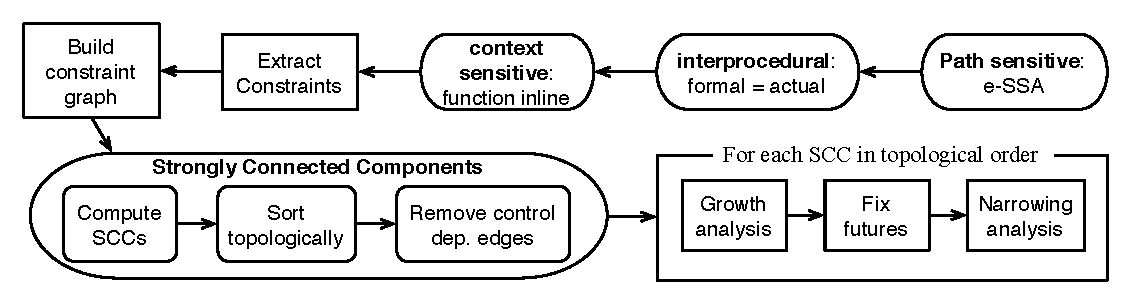
\includegraphics[width=1\textwidth]{images/algorithm}
\end{center}
\caption{\label{fig:algorithm}
Our implementation of range analysis.
Rounded boxes are optional steps.}
\end{figure}

\noindent
\textbf{Choosing a Program Representation.}
The solution to the range analysis problem in Figure~\ref{fig:ex1}
is imprecise because we did not take conditional tests into considerations.
Branches give us information about the ranges that some variables assume, but
only at {\em specific} program points.
For instance, given a test such as $(k_1 < 100)?$ in  Figure~\ref{fig:ex1}(b),
we know that $I[k_1] \sqsubseteq [-\infty, 99]$ whenever the condition is true.
In order to encode this information, we might split the live range of $k_1$
right after the branching point; thus, creating two new variables, one at the
path where the condition is true, and another where it is false.
There is a program representation, introduced by Bodik
{\em et al.}~\cite{Bodik00}, that performs this live range splitting:
the {\em Extended Static Single Assignment} form, or e-SSA for short.

Given that the exact rules to convert a program to e-SSA form have never been
explicitly stated in the literature, we describe our rules as follows.
Let $(v < c)?$ be a conditional test, and let $l_t$ and $l_f$ be labels in
the program, such that $l_t$ is the target of the test if the condition is true,
and $l_f$ is the target when the condition is false.
We split the live range of $v$ at any of these points if at least one of two
conditions is true:
(i) $l_f$ or $l_t$ dominate any use of $v$;
(ii) there exist a use of $v$ at the dominance frontier of $l_f$ or $l_t$.
For the notions of dominance and dominance-frontier, see Aho
{\em et al.}~\cite[p.656]{Aho06}.
To split the live range of $v$ at $l_f$ we insert at this
program point a copy $v_f = v \sqcap [c, +\infty]$, where $v_f$ is a fresh name.
We then rename every use of $v$ that is dominated by $l_f$ to $v_f$.
Dually, if we must split at $l_t$, then we create at this point a copy
$v_t = v \sqcap [-\infty, c-1]$, and rename variables accordingly.
If the conditional uses two variables, e.g., $(v_1 < v_2)?$, then we create
intersections bound to {\em futures}.
We insert, at $l_f$, $v_{1f} = v_1 \sqcap [\fun{ft}(v_2), +\infty]$,
and $v_{2f} = v_2 \sqcap [-\infty, \fun{ft}(v_1)]$.
Similarly, at $l_t$ we insert
$v_{1v} = v_1 \sqcap [-\infty, \fun{ft}(v_2) - 1]$
and $v_{2f} = v_2 \sqcap [\fun{ft}(v_1) + 1, +\infty]$.
Notice that a variable $v$ can never be associated with a future bound to
itself, e.g., $\fun{ft}(v)$.
This invariant holds because whenever the e-SSA conversion associates a variable
$u$ with $\fun{ft}(v)$, then $u$ is a fresh name created to split the live range
of $v$, given that $v$ was used in a conditional.

We use the notation $\fun{ft}(v)$ to denote the {\em future} bounds of a
variable.
As we will show in Section~\ref{sub:micro}, once the growth pattern of $v$ is
known, we can replace $\fun{ft}(v)$ by an actual value.
After splitting the live ranges according to the rules stated above, we might
have to insert $\phi$-functions into the transformed program to re-convert it to
SSA form.
This last step avoids that two different names given to the same original
variable be simultaneously {\em alive} at the program code.
A variable $v$ is alive at a program point $p$ if the program's control flow
graph contains a path from $p$ to a site where $v$ is used, that does not
go across any re-definition of $v$.
Figure~\ref{fig:ex_standard_eSSA}(a) shows our running example changed into
standard e-SSA form.
We have not created variable names for $i_f$ and $j_f$, because neither
$i_1$ nor $j_1$, the variables that have been renamed, are dominated by the
target of the conditional's else case.
In this example, new $\phi$-functions are not necessary: new variable
names are not alive together with the original variables.
The part (b) of this figure shows the solution that we get to this new
program.
The e-SSA form allows us to bind interval information directly to the live
ranges of variables; thus, giving us the opportunity to solve range analysis
sparsely.
More traditional approaches, which we call {\em dense analyses}, bind
interval information to pairs formed by variables and program points.

% TODO: check with Victor ** eSSA description could also say that we create sigmas even if lt/lf does not dominate any use of v (under some conditions), i.e. when there is a use in dominance frontier inside a phi function **

\begin{figure}[t!]
\begin{center}
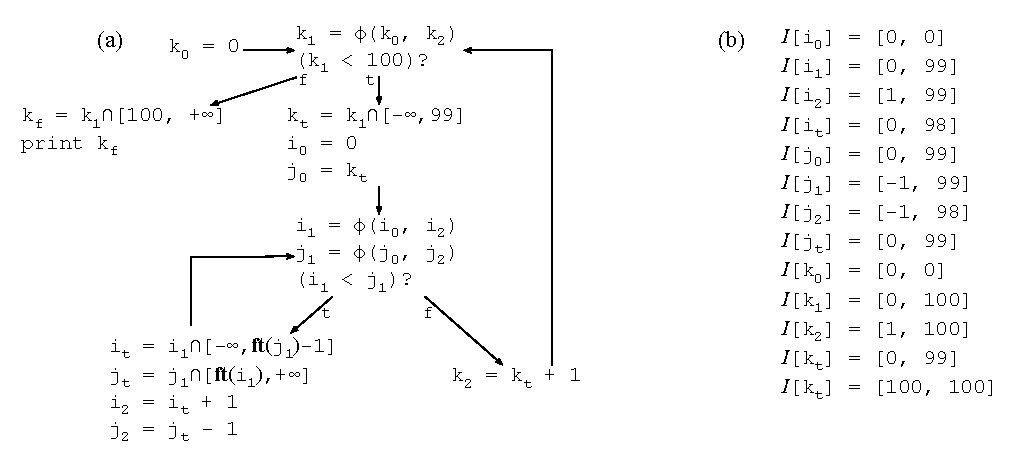
\includegraphics[width=0.9\textwidth]{images/ex_standard_eSSA}
\end{center}
\caption{\label{fig:ex_standard_eSSA}
(a) The control flow graph from Figure~\ref{fig:ex1}(b) converted to standard
e-SSA form.
(b) A solution to the range analysis problem
}
\end{figure}

%The standard e-SSA form serves well analysis that need range information
%at the use site of variables, such as conditional constant propagation,
%redundant code elimination and detection of buffer overflows.
%On the other hand, there exist compilation algorithms that require range
%information at the whole live range of variables.
%Examples of such algorithms include the family of
%bitwidth aware register allocators~\cite{Barik06,Pereira08,Tallam03} and
%hardware synthesizers~\cite{Cong05,Mahlke01,Stephenson00}.
%In order to provide extra precision to these algorithms, we may work with a
%non-pruned version of e-SSA form, which we produce by simply inserting copies
%after every conditional test, and then reconverting the entire program to
%SSA form.
%Figure~\ref{fig:ex_non_pruned} illustrates the difference between these two
%program representations.
%Notice that the non-pruned flavor might introduce dead variables in the
%program code, which can be removed by standard dead code elimination.

%\begin{figure}[t!]
%\begin{center}
%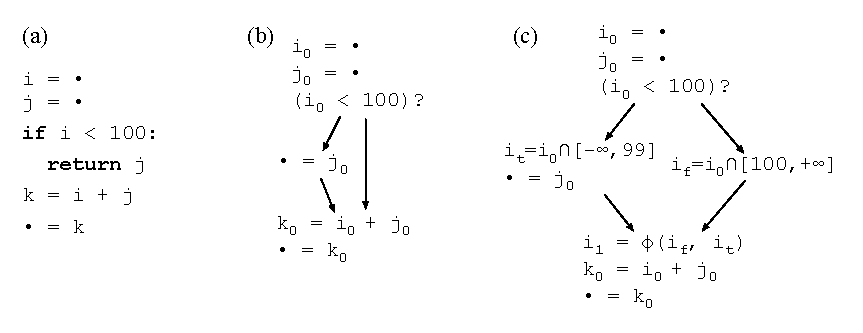
\includegraphics[width=0.9\textwidth]{images/ex_non_pruned}
%\end{center}
%\caption{\label{fig:ex_non_pruned}
%(a) Example program.
%(b) Standard e-SSA form.
%(c) Non-pruned e-SSA form.}
%\end{figure}

\noindent
\textbf{Extracting Constraints.}
Our implementation handles 18 different assembly instructions.
The constraints in Figure~\ref{fig:eval_function} show only a few examples.
Instructions that we did not show include, for instance, the multiplicative
operators \texttt{div} and \texttt{modulus},
the bitwise operators \texttt{and}, \texttt{or}, \texttt{xor} and \texttt{neg},
the different types of shifts, and the
logical operators \texttt{andalso}, \texttt{orelse} and \texttt{not}.
Most of these instructions are sign-agnostic; that is, given that numbers are
internally represented in 2's complement, the same implementation of a
constraint handles positive and negative numbers.
However, there are instructions that require different constraints, depending on
the input being signed or not.
Examples include \texttt{modulus} and \texttt{div}.
We also handle different kinds of type conversion, e.g., converting 8-bit
characters to 32-bit integers and vice-versa.
In addition to constraints that represent actual assembly instructions, we have
constraints to represent $\phi$-functions, and intersections, as seen in
Figure~\ref{fig:eval_function}.
The growth analysis that we will introduce in Section~\ref{sub:micro}
require monotonic transfer functions.
Many assembly operations, such as modulus or division, do not afford us
this monotonicity.
However, these non-monotonic instructions have conservative
approximations~\cite{Warren02}.

%Figure~\ref{fig:constraints} shows some examples of constraints that we
%derive from typical assembly instructions.
%
%\begin{figure}[t!]\begin{center}
%\begin{tabular}{|l@{\hspace{0.2cm}}l@{\hspace{0.3cm}}l|} \hline
%\textbf{Description} & \textbf{Operation} & \textbf{Constraint} \\ \hline
%Constant & $v = c$ & $V = [c, c]$ \\
%Assignment & $v_1 = v_2$ & $V_1 = V_2$ \\
%Multiplication & $v_1 = v_2 * c$ & $V_1 = c V_2$ \\
%Int. division & $v_1 = v_2 \ / \ v_3$ & $V_1 = V_2; V_1 = - V_2$ \\
%Modulus & $v_1 = v_2 \ \% \ c$ & $V_1 = [0, c - 1]$ \\
%Bitwise and & $v_1 = v_2 \ \& \ c$ & $V_1 = v_2 \sqcap [0, c]$ \\
%Bitwise or & $v_1 = v_2 \ | \ v_3$ & $V_1 = V_2 + V_3$ \\
%Left shift & $v_1 = v_2 \ \qside \ c$ & $V_1 = 2^c V_2$ \\ \hline
%\end{tabular}
%\end{center}
%\caption{\label{fig:constraints}Example of constraint derivation rules.
%We let $c$ denote a positive constant, $\{v, v_1, v_2\}$ are program
%variables and $\{V, V_1, V_2\} \subset \cal{V}$.}
%\end{figure}

\noindent
\textbf{The Constraint Graph.}
The main data structure that we use to solve the range analysis problem is
a variation of Ferrante {\em et al.}'s {\em program dependence
graph}~\cite{Ferrante87}.
For each constraint variable $V$ we create a variable node $N_v$.
For each constraint $C$ we create a constraint node $N_c$.
We add an edge from $N_v$ to $N_c$ if the name $V$ is used in $C$.
We add an edge from $N_c$ to $N_v$ if the constraint $C$ defines the name
$V$.
Figure~\ref{fig:ex_graph} shows the dependence graph that we build for the
e-SSA form program given in Figure~\ref{fig:ex_standard_eSSA}(a).
If $V$ is used by $C$ as the input of a future, then the edge from
$N_v$ to $N_c$ represents what Ferrante {\em et al.} call a {\em control
dependence}~\cite[p.323]{Ferrante87}.
We use dashed lines to represent these edges.
All the other edges denote {\em data dependences}~\cite[p.322]{Ferrante87}.

\begin{figure}[t!]
\begin{center}
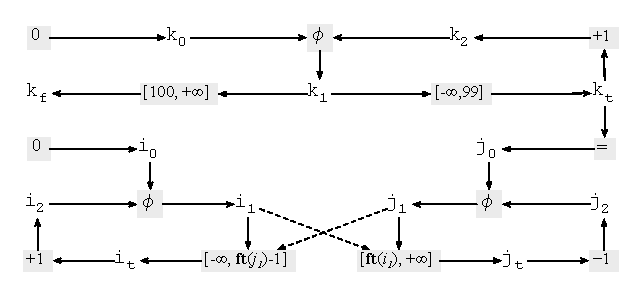
\includegraphics[width=0.7\textwidth]{images/ex_graph}
\end{center}
\caption{\label{fig:ex_graph}
The dependence graph that we build to the program in
Figure~\ref{fig:ex_standard_eSSA}.}
\end{figure}

\noindent
\textbf{Strongly Connected Components.}
To solve range analysis we find all the strongly connected components (SCCs) of
the dependence graph and collapse them into single nodes, obtaining a
directed acyclic graph.
We then sort the resulting DAG topologically, and apply the analyses from
Section~\ref{sub:micro} on every SCC in topological order.
Once we solve the range analysis problem for a SCC, we propagate the
intervals that we found to the variable nodes at the {\em frontier} of this
SCC.
A variable node $N_v$ is said to be in the frontier of a strongly connected
component $S$ if:
(i) $N_v \notin S$; and
(ii) there exists a variable node $N_v' \in S$, and a constraint node $N_c$,
such that $N_v \leftarrow N_c$, and $N_c \leftarrow N_v'$.
This propagation ensures that when analyzing a strongly connected component $S$
any influence that $S$ might suffer from nodes outside it has already been
considered.

When finding strongly connected components, we take control dependence
edges into consideration.
For instance, in Figure~\ref{fig:ex_graph} the nodes that correspond to the
variables $i_1$, $i_2$, $i_t$, $j_1$, $j_2$ and $j_t$ form a single component.
The dashed edges, which represent control dependences, keep all these variables
connected.
In this way, we ensure that, upon stumbling upon an interval associated with
future bounds, e.g., $\fun{ft}(v)$, either variable $v$ has been solved in a
previous component, or it belongs to the current component.
In the latter case, as we will see soon, we can still take $v$'s interval into
consideration.
This flexibility is possible because we first discover how each variable in
a strong component grows, before resolving future bounds.
As we show in Section~\ref{sub:showdown}, most of the strong components in
actual programs are singletons.
Furthermore, the composite components tend to be small.
These two facts ensure that the more costly parts of our algorithm only have to
handle small inputs.

\subsection{Finding Ranges in Strongly Connected Components}
\label{sub:micro}

Given a strongly connected component of the dependence graph with $N$ nodes,
we solve the range analysis problem in three-steps:
\begin{enumerate}
\item Run growth analysis: $O(N)$.

\item Fix intersections: $O(N)$.

\item Apply the narrowing operator: $O(N^2)$.

\end{enumerate}
However, before we start, we remove control dependence edges from the
strongly connected component, as they have no semantics to our transfer
functions.

\noindent
\textbf{Growth Analysis.}
The first step of our algorithm consists in determining how the interval bound
to each variable grows.
The possible behaviors of an interval are:
(i) does not change;
(ii) grows towards $+\infty$;
(iii) grows towards $-\infty$; and
(iv) grows in both directions.
We ensure termination of this phase via a {\em widening operator}.
We have experimented with four different widening strategies, which we
discuss in Section~\ref{sub:widen}.
One of these strategies is based on Cousot and Cousot's widening
operator~\cite[p.247]{Cousot77}.
The lattice of abstract states, plus a constraint system representing this
operator is given in Figure~\ref{fig:growth_analysis}.
Because the lattice has height three, the intervals bound to each variable can
change at most three times.

\begin{figure}[t!]
\begin{center}
\begin{tabular}{c@{\hspace{1.5cm}}c}
\begin{minipage}{2cm}
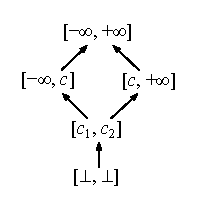
\includegraphics{images/growth_lattice}
\end{minipage}
&
\begin{minipage}{8cm}
\begin{small}
\begin{eqnarray*}
\begin{array}{c@{\hspace{0.5cm}}c}
\inferrule{I[Y] = [\bot, \bot]}{I[Y] \leftarrow e(Y)}
&
\inferrule{\lb{e(Y)} < \lb{I[Y]} \\ \ub{e(Y)} > \ub{I[Y]}}
{I[Y] \leftarrow [-\infty, +\infty ]}
\\
\\
\inferrule{\lb{e(Y)} < \lb{I[Y]}}
{I[Y] \leftarrow [-\infty, \ub{I[Y]}]}
&
\inferrule{\ub{e(Y)} > \ub{I[Y]}}
{I[Y] \leftarrow [\lb{I[Y]}, +\infty]}
\end{array}
\end{eqnarray*}
\end{small}
\end{minipage}
\end{tabular}
\end{center}
\caption{\label{fig:growth_analysis}
(Left) The lattice of the growth analysis.
(Right) Cousot and Cousot's widening operator. We evaluate the rules from
left-to-right, top-to-bottom, and stop upon finding a pattern matching.
Again: given an interval $\iota = [l, u]$, we let $\lb{\iota} = l$, and
$\ub{\iota} = u$}
\end{figure}

\begin{figure}[t!]
\begin{center}
\begin{eqnarray*}
\begin{array}{c}
\inferrule{Y = X \sqcap [l, \fun{ft}(V) + c] \\ \ub{I[V]} = u}
{Y = X \sqcap [l, u + c]} \mbox{\hspace{0.3cm}} u, c \in \mathbb{Z} \cup \{-\infty, +\infty\}
\\
\\
\inferrule{Y = X \sqcap [\fun{ft}(V) + c, u] \\ \lb{I[V]} = l}
{Y = X \sqcap [l + c, u]} \mbox{\hspace{0.3cm}} l, c \in \mathbb{Z} \cup \{-\infty, +\infty\}
\end{array}
\end{eqnarray*}
\end{center}
\caption{\label{fig:fix_intersects}Rules to replace futures by actual
bounds.}
\end{figure}

%\begin{figure}[t!]
%\begin{equation*}
%S[X] \leftarrow
%\begin{cases}
%``\ ? \ " \ \ \mbox{if} \ I[X] = [-\infty, +\infty]\\
%``\downarrow" \ \mbox{if} \ I[X] = [-\infty, c], c \in \mathbb{Z} \\
%``\uparrow" \ \mbox{if} \ I[X] = [c, +\infty],  c \in \mathbb{Z} \\
%`` \ 0 \ " \ \ \mbox{if} \ I[X] = [c_1, c_2], c_1, c_2 \in \mathbb{Z}
%\end{cases}
%\end{equation*}
%\caption{\label{fig:st_mem}The growth state of each variable.}
%\end{figure}

\begin{figure}[t!]
\begin{center}
\begin{eqnarray*}
\begin{array}{c@{\hspace{0.9cm}}c}
\inferrule{\lb{I[Y]} = -\infty \\ \lb{e(Y)} > -\infty}
{I[Y] \leftarrow [\lb{e(Y)}, \ub{I[Y]}]}
&
\inferrule{\lb{I[Y]} > \lb{e(Y)}}
{I[Y] \leftarrow [\lb{e(Y)}, \ub{I[Y]}]}
\\
\\
\inferrule{\ub{I[Y]} = +\infty \\ \ub{e(Y)} < +\infty}
{I[Y] \leftarrow [\lb{I[Y]}, \ub{e(Y)}]}
&
\inferrule{\ub{I[Y]} < \ub{e(Y)}}
{I[Y] \leftarrow [\lb{I[Y]}, \ub{e(Y)}]}
\end{array}
\end{eqnarray*}
\end{center}
\caption{\label{fig:crop_analysis}Cousot and Cousot's narrowing operator.}
\end{figure}

\noindent
\textbf{Fixing futures.}
The ranges found by the growth analysis tells us which variables have fixed
bounds, independent on the intersections in the constraint system.
Thus, we can use actual limits to replace intersections bounded by futures.
Figure~\ref{fig:fix_intersects} shows the rules to perform these substitutions.
In order to correctly replace a future $\fun{ft}(v)$ that limits a variable
$v'$, we need to have already applied the growth analysis onto $v$.
Had we considered only data dependence edges, then it would be possible
that $N_{v'}$ be analyzed before $N_v$.
However, because of control dependence edges, this case cannot happen.
The control dependence edges ensure that any topological ordering of the
constraint graph either places $N_v$ before $N_{v'}$, or places these nodes
in the same strongly connected component.
For instance, in Figure~\ref{fig:ex_graph}, variables $j_1$ and $i_t$ are in
the same SCC only because of the control dependence edges.

\noindent
\textbf{Narrowing Analysis.}
The growth analysis associates very conservative bounds to each variable.
Thus, the last step of our algorithm consists in narrowing these intervals.
We accomplish this step via Cousot and Cousot's classic narrowing
operator~\cite[p.248]{Cousot77}, which we show in
Figure~\ref{fig:crop_analysis}.

\begin{figure}[t!]
\begin{center}
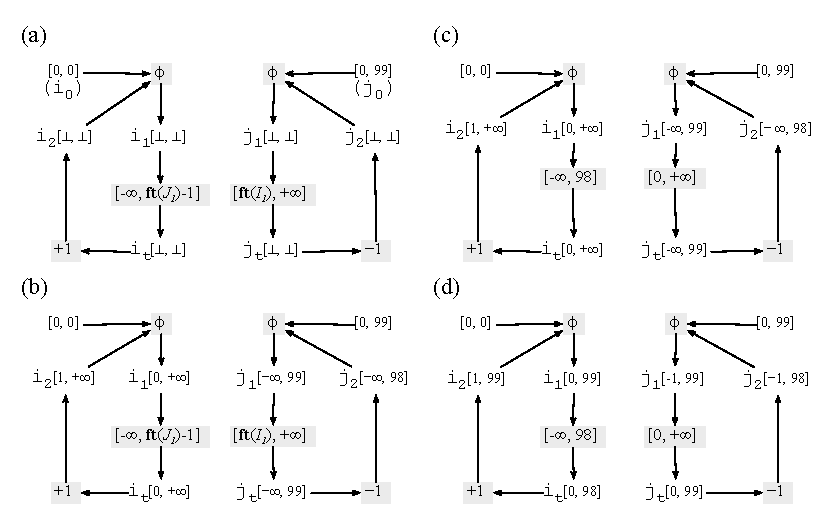
\includegraphics[width=\textwidth]{images/ex_partition_grow_crop}
\end{center}
\caption{\label{fig:ex_partition_grow_crop}
Four snapshots of the last SCC of Figure~\ref{fig:ex_standard_eSSA}.
(a) After removing control dependence edges.
(b) After running the growth analysis.
(c) After fixing the intersections bound to futures.
(d) After running the narrowing analysis.}
\end{figure}

% TODO: check if we say fix point or fixed point.
\noindent
\textbf{Example:}
Continuing with our example, Figure~\ref{fig:ex_partition_grow_crop} shows
the application of our algorithm on the last strong component of
Figure~\ref{fig:ex_graph}.
We are not guaranteed to find the least fixed point of a constraint system.
However, in this example we did it.
Figure~\ref{fig:ex_standard_eSSA}(b) shows our final solution for this example.
This solution is very precise, in the sense that it is the least fixed
point of the constraint system given in Figure~\ref{fig:eval_function}.
However, the solution is still an over approximation of the dynamic behavior of
the program in Figure~\ref{fig:ex1}(a).
For instance, we have found that variable $i$ could reach the upper value of
99.
In any actual run of the program, $i$ could be at most 50.
Analyses on relational lattices, such as the polyhedron~\cite{Cousot78} or the
Octagon~\cite{Mine06} domains, can infer such tighter bounds, as shown by
Lakhdar-Chaouch {\em et al.}~\cite{Lakhdar11}.
However, analyses on these higher dimensional domains are much more
computationally expensive than analyses on the interval domain~\cite{Oh12}.

We emphasize that finding this tight solution was only possible because of
the topological ordering of the constraint graph in Figure~\ref{fig:ex_graph}.
Upon meeting the constraint graph's last SCC, shown in
Figure~\ref{fig:ex_partition_grow_crop}, we had already determined that the
interval $[0, 0]$ is bound to $i_0$ and that the interval $[0, 99]$ is bound to
$j_0$, as we show in Figure~\ref{fig:ex_partition_grow_crop}(a).
Had we applied the widening operator onto the whole graph, then we would
have found out that variable $j_1$ is bound to $[-\infty, +\infty]$.
This imprecision happens because, on one hand $j_1$'s interval is influenced
by $k_t$'s, which is upper bounded by $+\infty$.
On the other hand $j_1$ is part of a decreasing cycle of dependences formed by
variables $j_t$ and $j_2$ in addition to itself.
Therefore, if we had applied the widening phase over the entire program followed
by a global narrowing phase, then we would not be able to recover some of
widening's precision loss.
However, because in this example we only analyze $j$'s SCC after we have
analyzed $k$'s, $k$ only contribute the constant range $[0, 99]$ to $j_0$.


%%%%%%%%%%%%%%%%%%%%%%%%%%%%%%%%%%%%%%%%%%%%%%%%%%%%%%%%%%%%%%%%%%%%%%%%%%%%%%%%
\subsection{Range Analysis Showdown}
\label{sub:showdown}

The objective of this section is to show, via experimental numbers, that our
implementation of range analysis is fast, economic and effective.
We have used it to analyze a test suite with 2.72 million lines of C code,
which includes, in addition to all the benchmarks distributed with LLVM,
the programs in the SPEC CPU 2006 collection.

\noindent
\textbf{Time and Memory Complexity.}
Figure~\ref{fig:TimeCorr} provides a visual comparison between the time to
run our algorithm and the size of the input programs.
We show data for the 100 largest benchmarks in our test suite, in number
of variable nodes in the constraint graph.
We perform function inlining before running our analysis.
Each point in the X line corresponds to a benchmark.
We analyze the smallest benchmark in this set, \texttt{Prolangs-C/deriv2}, which
has 1,131 variable nodes in the constraint graph, in 20ms.
We take 15.91 sec to analyze our largest benchmark, \texttt{403.gcc}, which,
after function inlining, has 1,266,273 assembly instructions, and a
constraint graph with 679,652 variable nodes.
For this data set, the coefficient of determination $(R^2)$ is 0.967, which
provides very strong evidence about the linear asymptotic complexity of our
implementation.

\begin{figure}[t!]
\begin{center}
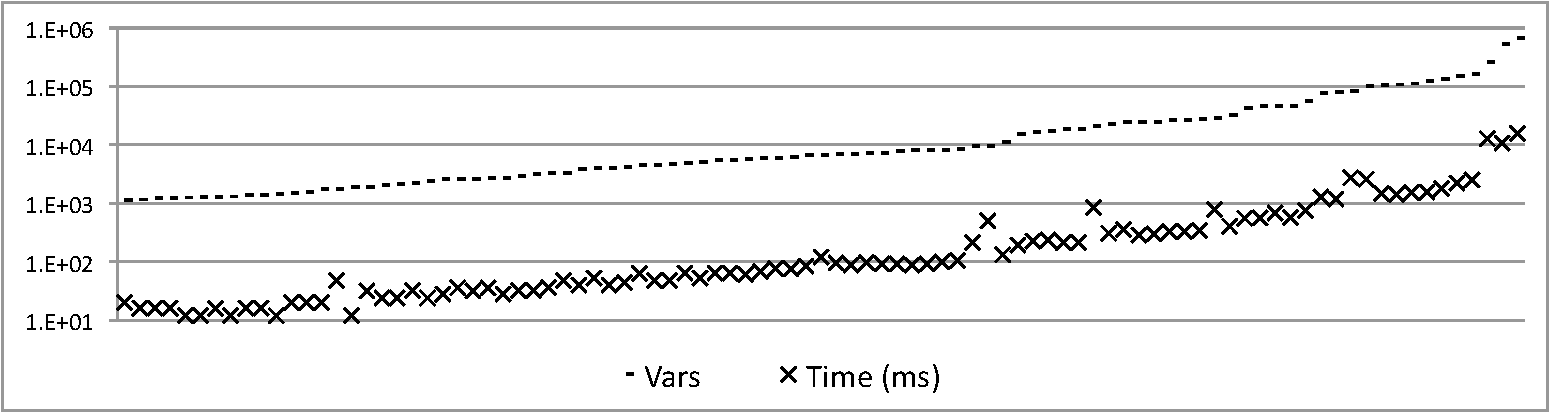
\includegraphics[width=0.9\textwidth]{images/TimeCorr}
\end{center}
\caption{\label{fig:TimeCorr}
Correlation between program size (number of var nodes in constraint
graphs after inlining) and analysis runtime (ms).
Coefficient of determination = 0.967.
}
\end{figure}

The experiments also reveal that the memory consumption of our implementation
is linear with the program size.
Figure~\ref{fig:MemCorr} plots these two quantities together.
The linear correlation, in this case, is even stronger than that found in
Figure~\ref{fig:TimeCorr}, which compares runtime and program size: the
coefficient of determination is 0.9947.
The figure only shows our 100 largest benchmarks.
Again, SPEC \texttt{403.gcc} is the heaviest benchmark, requiring
265,588KB to run.
Memory includes stack, heap and the executable program code.

\begin{figure}[t!]
\begin{center}
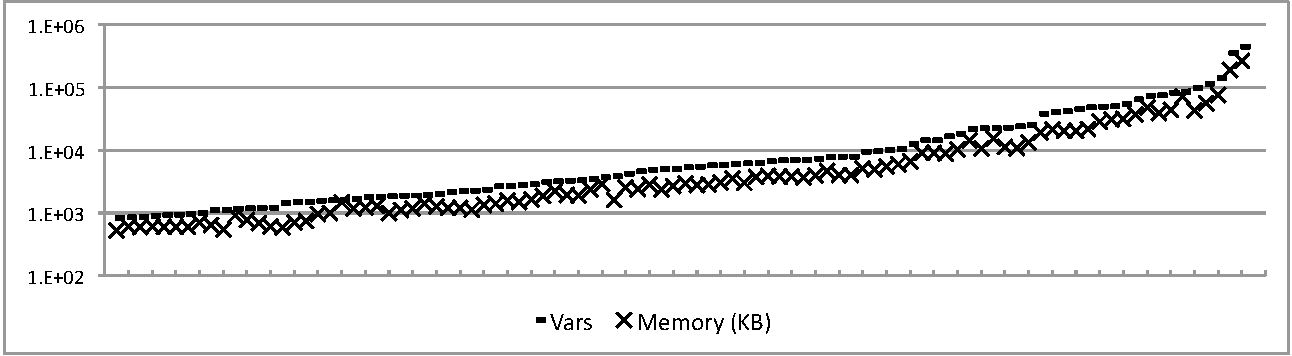
\includegraphics[width=0.9\textwidth]{images/MemCorr}
\end{center}
\caption{\label{fig:MemCorr}
Comparison between program size (number of var nodes in constraint
graphs) and memory consumption (KB).
Coefficient of determination = 0.9947.
}
\end{figure}

\noindent
\textbf{Precision.}
Our implementation of range analysis is remarkably precise, considering its
runtime.
Lakhdar {\em et al.}'s relational analysis~\cite{Lakhdar11}, for instance, takes
about 25 minutes to go over a program with almost 900 basic blocks.
We analyze programs of similar size in less than one second.
We do not claim our approach is as precise as such algorithms, even though we
are able to find exact bounds to 4/5 of the examples presented
in~\cite{Lakhdar11}.
On the contrary, this paper presents a compromise between precision and speed
that scales to very large programs.
Nevertheless, our results are far from being trivial.
We have implemented a dynamic profiler that measures, for each variable,
its upper and lower limits, given an execution of the target program.
Figure~\ref{fig:precision} compares our results with those measured
dynamically for the Stanford benchmark suite, which is publicly
available~\footnote{\texttt{http://classes.engineering.wustl.edu/cse465/docs/BCCExamples/stanford.c}}.
We chose Stanford because these benchmarks do not read data from external
files; hence, imprecisions are due to library functions that we cannot
analyze.

\begin{figure}[t!]
\begin{center}
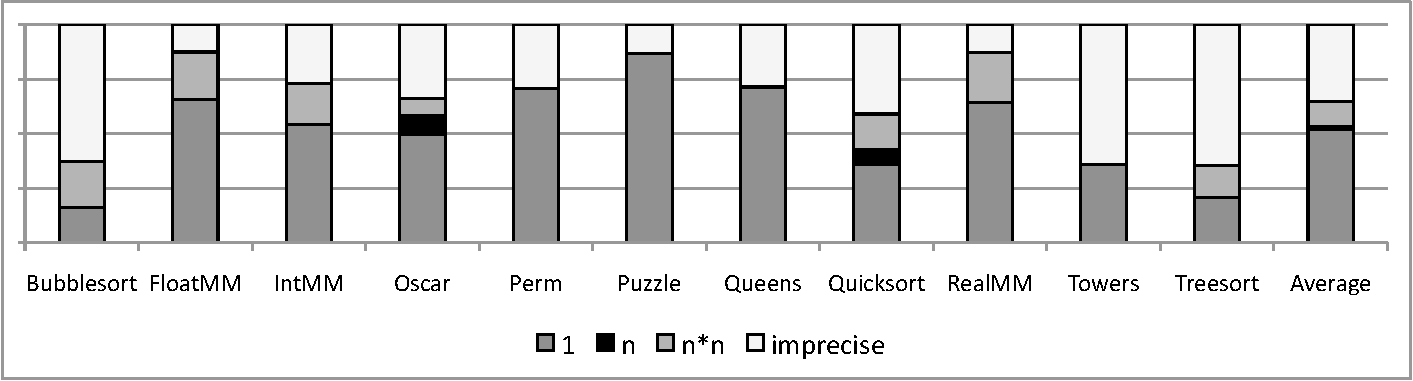
\includegraphics[width=0.97\textwidth]{images/precUpperBound}
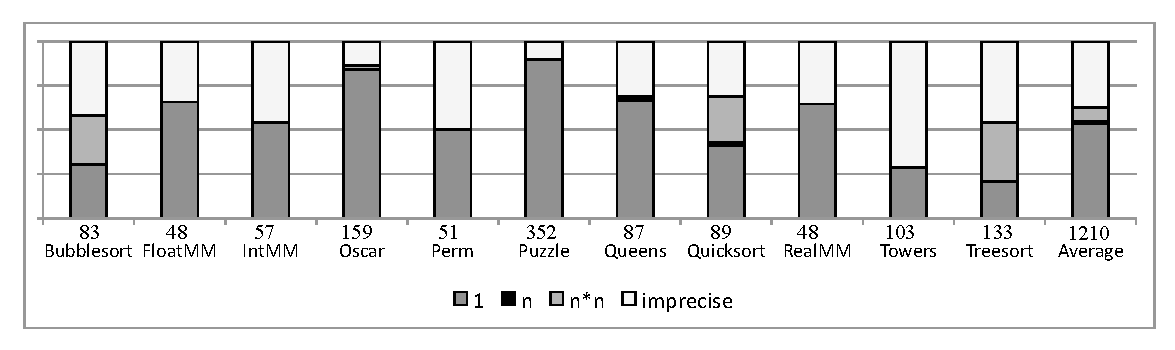
\includegraphics[width=\textwidth]{images/precLowerBound}
\end{center}
\caption{\label{fig:precision}
(Upper) Comparison between static range analysis and dynamic profiler for
upper bounds.
(Lower) Comparison between static range analysis and dynamic profiler for
lower bounds. The numbers above the benchmark names give the number of
variables in each program.}
\end{figure}

We have classified the bounds estimated by the static analysis into four
categories.
The first category, which we call $1$, contains those bounds that are tight:
during the execution of the program, the variable has been assigned an upper,
or lower limit, that equals the limit inferred statically.
The second category, which we call $n$, contains the bounds that are
within twice the value inferred statically.
For instance, if the range analysis estimates that a variable $v$ is in the
range $[0, 100]$, and during the execution the dynamic profiler finds that
its maximum value is $51$, then $v$ falls into this category.
The third category, $n^2$, contains variables whose actual value is within
a quadratic factor from the estimated value.
In our example, $v$'s upper bound would have to be at most $10$ for it to
be in this category.
Finally, the fourth category contains variables whose estimated value lays
outside a quadratic factor of the actual value.
We call this category {\em imprecise}, and it contains mostly the limits that
our static analysis has marked as either $+\infty$ or $-\infty$.

As we see in Figure~\ref{fig:precision}, 54.11\% of the lower limits that
we have estimated statically are exact.
Similarly, 51.99\% of our upper bounds are also tight.
The figure also shows that, on average, 37.39\% of our lower limits are
imprecise, and 35.40\% of our upper limits are imprecise.
This result is on pair with those obtained by more costly analysis, such as
Stephenson {\em et al.}'s~\cite{Stephenson00}.
However, whereas that approach has only been tested on single functions,
we have been able to deal with remarkably larger programs.

%mmmmmmmmmmmmmmmmmmmmmmmmmmmmmmmmmmmmmmmmmmmmmmmmmmmmmmmmmmmmmmmmmmmmmmmmmmmmmm
\section{Design Space}
\label{sec:design}

As we see from a cursory glance at Figure~\ref{fig:algorithm}, our range
analysis algorithm has many optional modules.
These modules give the user the chance to choose between more precise results,
or a faster analysis.
Given the number of options, the design space of a range analysis algorithm
is vast.
In this section we try to cover some of the most important tradeoffs.
Figure~\ref{fig:space} plots, for the integer programs in the SPEC CPU 2006
benchmark suite, precision versus speed for different configurations of
our implementation.
Our initial goal when developing this analysis was to support a bitwidth-aware
register allocator.
Thus, we measure precision by the average number of bits that our
analysis allows us to save per program variable.
It is very important to notice that we do not consider constants in our statistics of precision.
In other words, we only measure bitwidth reduction in variables that a constant
propagation step could not remove.


\begin{figure}[t!]
\begin{center}
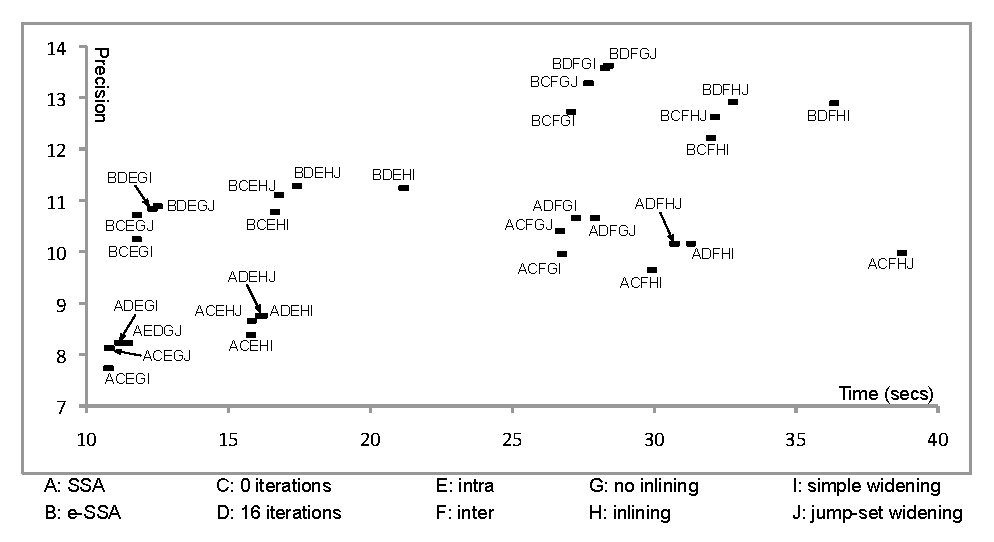
\includegraphics[width=\textwidth]{images/space}
\end{center}
\caption{\label{fig:space}
Design space exploration: precision (percentage of bitwidth reduction)
versus speed (secs) for different configurations of our algorithm analyzing
the SPEC CPU 2006 integer benchmarks.}
\end{figure}

\subsection{Strongly Connected Components}
\label{sub:sccs}

The greatest source of improvement in our implementation is the use of strongly
connected components.
In order to propagate ranges across the constraint graph, we fragment it
into strongly connected components, collapse each of these components into
single nodes, and sort the resulting directed acyclic graph topologically.
We then solve the range analysis problem for each component individually.
Once we have solved a component, we propagate its ranges to the next
components, and repeat the process until we walk over the entire constraint
graph.
It is well-known that this technique is essential to speedup constraint solving
algorithms~\cite[Sec 6.3]{Nielson99}.
In our case, the results are dramatic, mostly in terms of speed, but also in
terms of precision.
Figure~\ref{fig:impactSCC} shows the speedup that we gain by using strong
components.
We show results for the integer programs in the SPEC CPU 2006 benchmark suite.
In some cases, as in \texttt{xalancbmk} the analysis on strong components is
450x faster.

\begin{figure}[t!]
\begin{center}
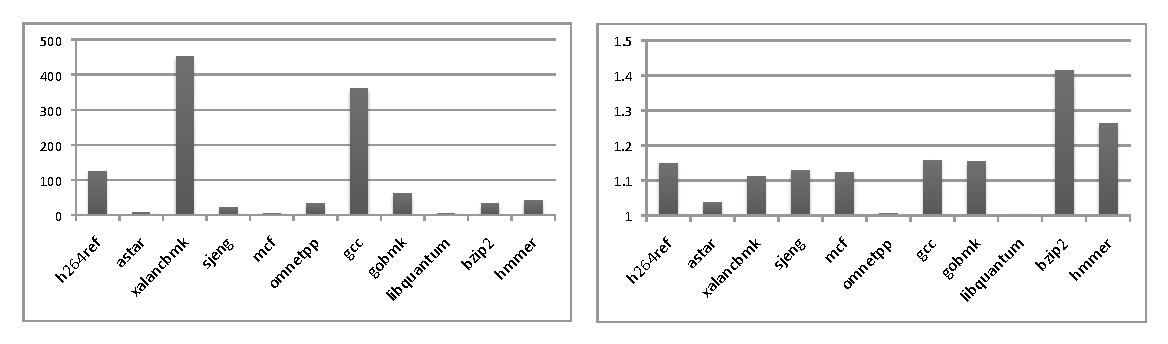
\includegraphics[width=\textwidth]{images/impactSCC}
\end{center}
\caption{\label{fig:impactSCC}
(Left) Time to run our analysis without building strong components
divided by time to run the analysis on strongly connected components.
(Right) Precision, in bitwidth reduction, that we obtain with strong
components, divided by the precision that we obtain without them.
}
\end{figure}

The strong components improve the precision of our growth analysis.
According to Figure~\ref{fig:impactSCC}, in some cases, as in \texttt{bzip2},
strong components increase our precision by 40\%.
The gains in precision happen because, by completely resolving a component,
we are able to propagate constant intervals to the next components, instead
of propagating intervals that can grow in both directions.
As an example, in Figure~\ref{fig:ex_partition_grow_crop} we pass the range
$[0, 99]$ from variable $k$ to the component that contains variable $j$.
Had we run the analysis in the entire constraint graph, by the time we
applied the growth analysis on $j$ we would still find $k$ bound to
$0, +\infty$.


\subsection{The choice of a program representation}
\label{sub:program_rep}

If strong components account for the largest gains in speed, the choice of
a suitable program representation is responsible for the largest gains in
precision.
However, here we no longer have a win-win condition: a more expressive
program representation decreases our speed, because it increases the
size of the target program.
We have tried our analysis in two different program representations: the
Static Single Assignment (SSA) Form~\cite{Cytron91}, and the Extended Static
Single Assignment (e-SSA) form~\cite{Bodik00}.
The SSA form gives us a faster, albeit more imprecise, analysis.
Any program in e-SSA form has also the SSA core property: any variable name
has at most one definition site.
The contrary is not true: SSA form programs do not have the core e-SSA
property: any use site of a variable that appears in a conditional test
post-dominates its definition.
The program in Figure~\ref{fig:ex1}(b) is in e-SSA form.
The live ranges of variables $i_1$ and $j_1$ have been split right after the
conditional test via the assertions that creates variables $i_t$ and $j_t$.
The e-SSA format serves well analyses that extract information from definition
sites and conditional tests, and propagate this information forwardly.
Examples include, in addition to range analysis, tainted flow
analysis~\cite{Rimsa11} and array bounds checks elimination~\cite{Bodik00}.

\begin{figure}[t!]
\begin{center}
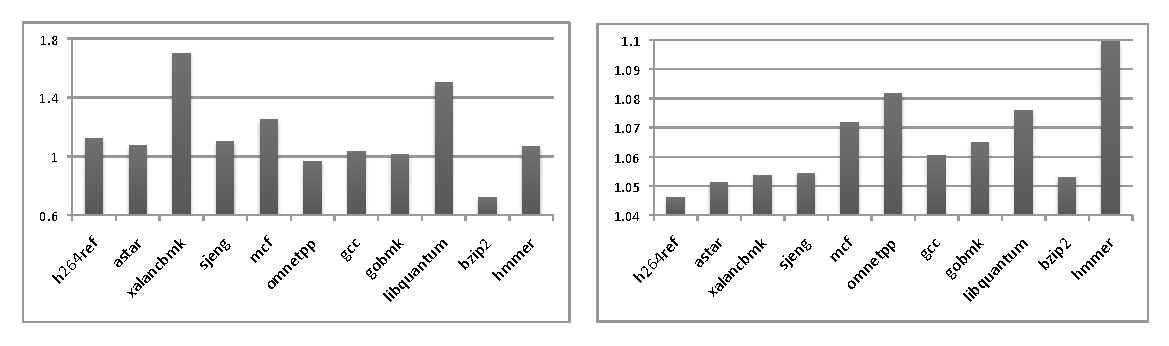
\includegraphics[width=1\textwidth]{images/impactESSA}
\end{center}
\caption{\label{fig:impactESSA}
(Left) Bars give the time to run analysis on e-SSA form programs divided by
the time to run analysis on SSA form programs.
(Right) Bars give the size of the e-SSA form program, in number of
assembly instructions, divided by the size of the SSA form program.}
\end{figure}

Figure~\ref{fig:impactESSA} compares these two program representations in
terms of runtime.
As we see in Figure~\ref{fig:impactESSA}(Left), the e-SSA form slows down our
analysis.
In some cases, as in \texttt{xalancbmk}, this slowdown increases execution
time by 71\%.
Runtime increases for two reasons.
Firstly, the e-SSA form programs are larger than the SSA form programs, as we
show in Figure~\ref{fig:impactESSA}(Right).
However, this growth is small: in none of the integer programs in SPEC
CPU 2006 we verified an increase in code size of more than 9\%.
Secondly, the e-SSA form program has futures; hence requiring the future
resolution phase of our algorithm, which is not necessary in SSA form programs.
Nevertheless, if the e-SSA form slowdowns the analysis runtime, its gains in precision
are remarkable, as seen in Figure~\ref{fig:precESSA}.
These gains happen because the e-SSA format lets the analysis to use the
results of conditional tests to narrow the ranges of variables.

\begin{figure}[t!]
\begin{center}
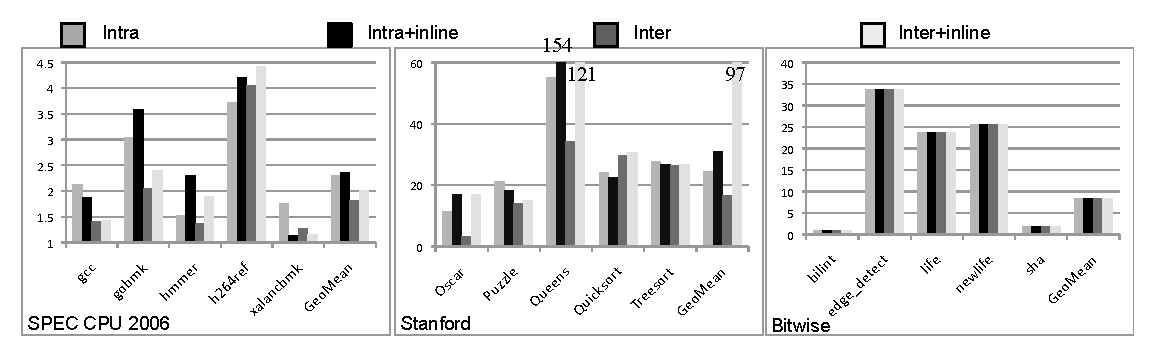
\includegraphics[width=1\textwidth]{images/precESSA}
\end{center}
\caption{\label{fig:precESSA}
The impact of the e-SSA transformation on precision for three different
benchmark suites. Bars give the ratio of precision (in bitwidth reduction),
obtained with e-SSA form conversion divided by precision without e-SSA form
conversion.}
\end{figure}

\subsection{Intra versus Inter-procedural Analysis}
\label{sub:whole}

A naive implementation of range analysis would be intra-procedural; that is,
would solve the range analysis problem once per each function.
However, we can gain in precision by performing it inter-procedurally.
An inter-procedural implementation allows the results found for a function $f$
to flow into other functions that $f$ calls.
Figure~\ref{fig:intra} illustrates the inter-procedural analysis for the
program seen in Figure~\ref{fig:ex1}(a).
The trivial way to produce an inter-procedural implementation is to insert
into the constraint system assignments from the actual parameter names to the
formal parameter names.
In our example of Figure~\ref{fig:intra}, our constraint graph contains a flow
of information from $0$, the actual parameter, to $k_0$, the formal parameter
of function \texttt{foo}.

\begin{figure}[t!]
\begin{center}
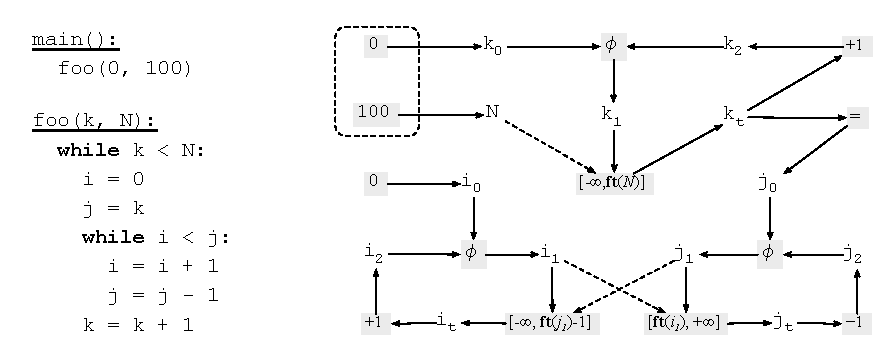
\includegraphics[width=\textwidth]{images/intra}
\end{center}
\caption{\label{fig:intra}
Example where an intra-procedural implementation would lead to imprecise
results.
}
\end{figure}

Figure~\ref{fig:wholeImpact} compares the precision of the intra and
inter-procedural analyses for the five largest programs in three different
categories of benchmarks: SPEC CPU 2006, the Stanford Suite~\footnote{\texttt{http://classes.engineering.wustl.edu/cse465/docs/BCCExamples/stanford.c}} and
Bitwise~\cite{Stephenson00}.
Our results for the SPEC programs were disappointing: on the average for
the five largest programs, the intra-procedural version of our analysis saves
5.23\% of bits per variable.
The inter-procedural version increases this number to 8.89\%.
A manual inspection of the SPEC programs reveals that this result is expected:
these programs manipulate files, and their source codes do not provide enough
explicit constants to power our analysis up.
However, with numerical benchmarks we fare much better.
On the average our inter-procedural algorithm reduces the bitwidth of the
Stanford benchmarks by 36.24\%.
For Bitwise we obtain a bitwidth reduction of 12.27\%.
However, this average is lowered by two outliers: \texttt{edge\_detect} and
\texttt{sha}, which have been purposely engineered to be resilient against
range analyses~\cite{Stephenson00}.
The bitwise benchmarks were implemented by Stephenson
{\em et al.}~\cite{Stephenson00} to validate their intra-procedural bitwidth
analysis.
Our results are on par with those found by the original authors.
The bitwise programs contain only the \texttt{main} function; thus, different
versions of our algorithm find the same results when applied onto these
programs.

\subsection{Achieving Partial Context-Sensitiveness via Function Inlining}
\label{sub:context}

Another way to increase the precision of range analysis is via a
context-sensitive implementation.
Context-sensitiveness allows us to distinguish different calling sites of
the same function.
Figure~\ref{fig:context} shows why the ability to make this distinction is
important for precision.
In Figure~\ref{fig:context}(a) we have two different calls of function
\texttt{foo}.
If we apply the trivial inter-procedural approach of Section~\ref{sub:whole},
then we get the graph shown in Figure~\ref{fig:context}(b).
In other words, if a function is called more than once, then its formal
parameters will receive information from many actual parameters.
We use $\phi$-functions to bind this information together into a single
flow.
However, in this case the multiple assignment of values to parameters
makes the ranges of these parameters very large, whereas in reality they
are not.
A way to circumvent this source of imprecision is via function inlining,
as we show in Figure~\ref{fig:context}(c).
The results that we can derive for the transformed program are more
precise, as each input parameter is assigned a single value.

\begin{figure}[t!]
\begin{center}
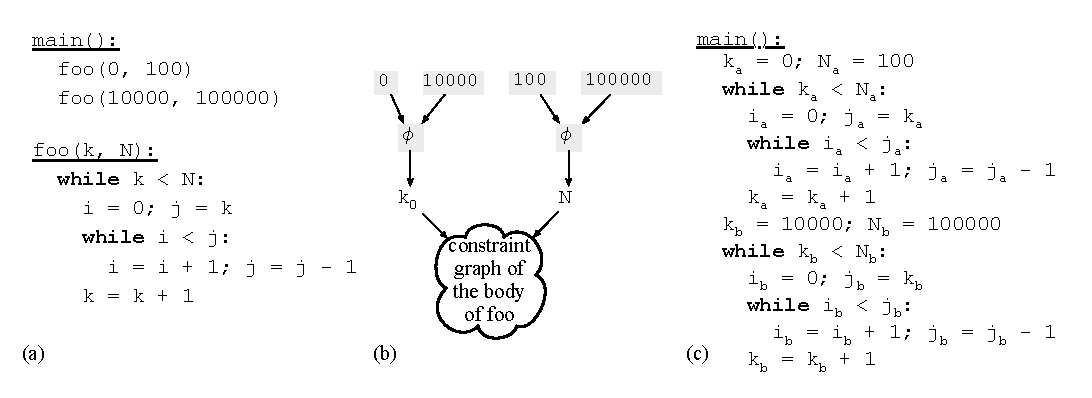
\includegraphics[width=\textwidth]{images/context}
\end{center}
\caption{\label{fig:context}
Example where a context-sensitive implementation improves the results of
range analysis.
}
\end{figure}

Figure~\ref{fig:wholeImpact} also shows how function inlining modifies the
precision of our results.
It is difficult to find an adequate way to compare the precision of
our analysis with, and without inlining.
This difficulty stems from the fact that this transformation tends to change
the target program too much.
In absolute numbers, we always reduce the bitwidth of more variables after
function inlining.
However, proportionally function inlining leads to a smaller percentage of
bitwidth reduction for many benchmarks.
In the Stanford Collection, for instance, where most of the functions are
called in only one location, inlining leads to worse precision results.
On the other hand, for the SPEC programs, inlining, even in terms of
percentage of reduction, tends to increase our measure of precision.

\begin{figure}[t!]
\begin{center}
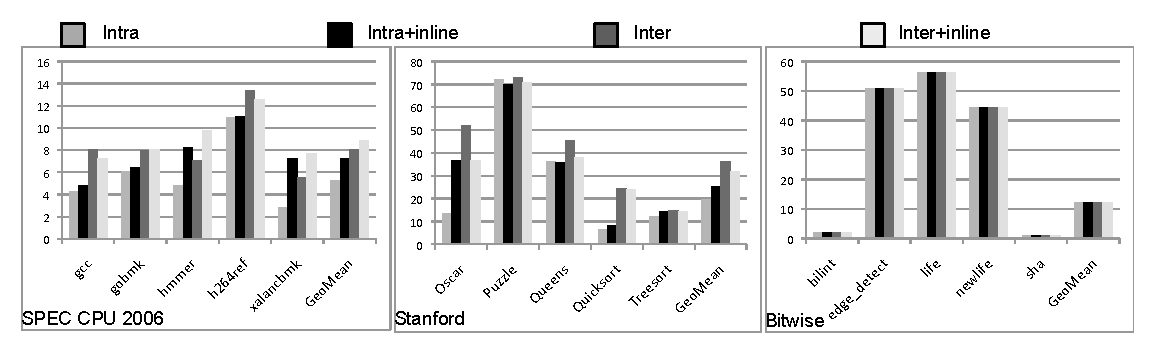
\includegraphics[width=\textwidth]{images/wholeImpact}
\end{center}
\caption{\label{fig:wholeImpact}
The impact of inter-procedural analysis on precision. Each bar shows precision
in \%bitwidth reduction.}
\end{figure}

\noindent
\textbf{Intra vs Inter-procedural runtimes.}
Figure~\ref{fig:timeComp}(Left) compares three different execution modes.
Bars are normalized to the time to run the intra-procedural analysis
without inlining.
On the average, the intra-procedural mode is 28.92\% faster than the
inter-procedural mode.
If we perform function inlining, then this difference is 45.87\%.
These numbers are close because our runtime is bound to the
size of the strong components.
Although function inlining can increase the number of strongly connected
components in the constraint graph, it cannot increase the size of the largest
component, when compared to the simple inter-procedural analysis of
Section~\ref{sub:whole}.

\begin{figure}[t!]
\begin{center}
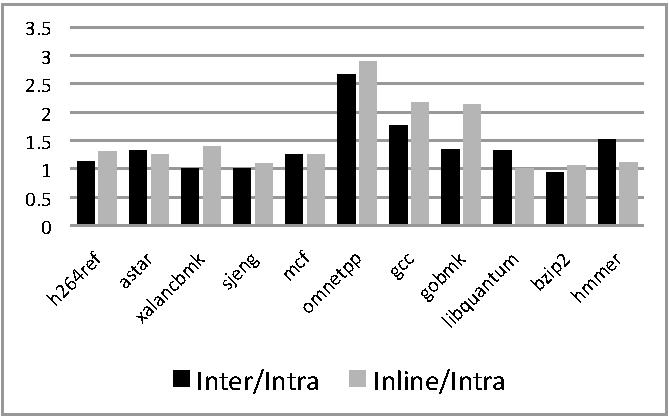
\includegraphics[width=0.45\textwidth]{images/timeIntraInterInline}
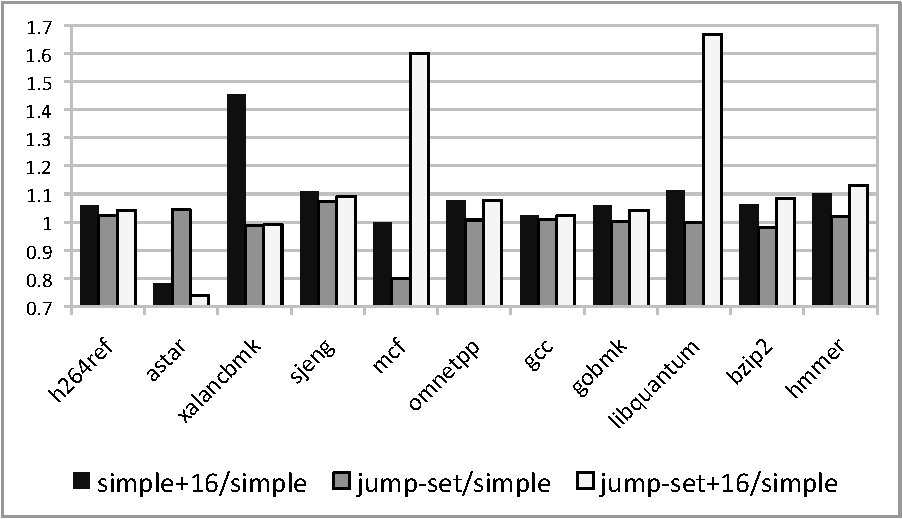
\includegraphics[width=0.485\textwidth]{images/timeWideningOperators}
\end{center}
\caption{\label{fig:timeComp}
(Left) Runtime comparison between intra, inter and inter+inline versions of
our algorithm.
(Right) Runtime comparison between different widening operators.
The bars are normalized to the time to run the intra-procedural analysis.
}
\end{figure}

\subsection{Choosing a Widening Strategy}
\label{sub:widen}

We have implemented the widening operator used in the growth analysis in
two different ways.
The first way, which we call {\em simple}, is based on Cousot and
Cousot's original widening operator~\cite{Cousot77}, and we have shown it
in Figure~\ref{fig:growth_analysis}(Right).
The second widening strategy, which we call {\em jump-set widening} consists
in using the constants that appear in the program text, in sorted order, as
the next limits of each interval after widening is applied.
This operator is common in implementations of range
analysis~\cite[p.228]{Nielson99}.
Jump-set widening never produces worse results than the simple operator, and
sometimes it does better.
Figure~\ref{fig:jumpSet} shows an example taken from the code of
SPEC CPU \texttt{bzip2}.
Part of the constraint graph of the program in Figure~\ref{fig:jumpSet}(a)
is given in Figure~\ref{fig:jumpSet}(b).
The result of applying the simple operator is shown in
Figure~\ref{fig:jumpSet}(c).
Jump-set widening would use the lattice in Figure~\ref{fig:jumpSet}(d),
instead of the lattice in Figure~\ref{fig:growth_analysis}(Left).
This lattice yields the result given in Figure~\ref{fig:jumpSet}(e),
which is more precise.

\begin{figure}[t!]
\begin{center}
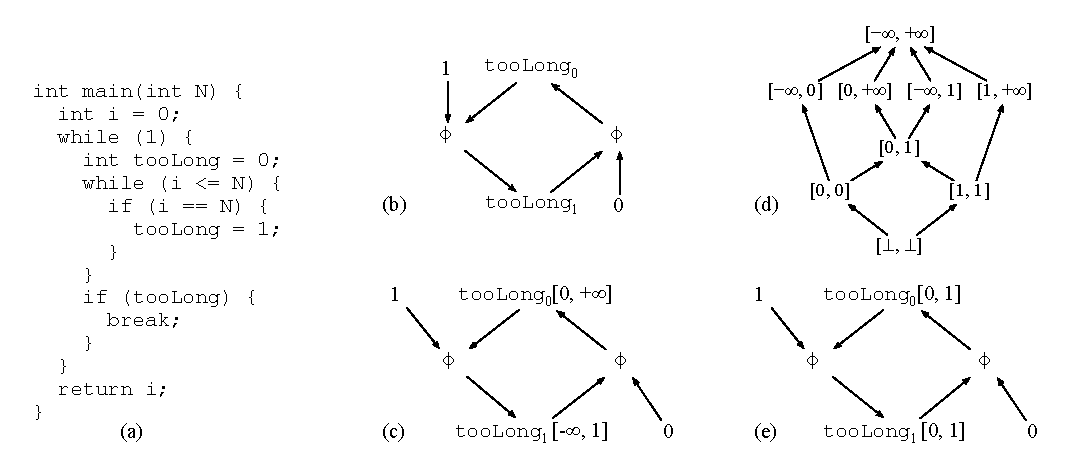
\includegraphics[width=1\textwidth]{images/jumpSet}
\end{center}
\caption{\label{fig:jumpSet}
An example where jump-set widening is more precise.}
\end{figure}

%%%%%%%%%%%%%%%%%%%%%%%%%%%%%%%%%%%%%%%%%%%%%%%%%%%%%%%%%%%%%%%%%%%%%%%%%%%%%%%%
Another way to improve the precision of growth analysis is to perform a few
rounds of abstract interpretation on the constraint graph, and, in case the
process does not reach a fixed point, only then to apply the widening operator.
Each round of abstract interpretation consists in evaluating all the
constraints, and then updating the intervals that change from one evaluation to
the other.
For instance, in Figure~\ref{fig:jumpSet} one round of abstract interpretation,
coupled with the simple widening operator, would be enough to reach the
fixed point of that constraint system.
We have experimented with 0 and 16 iterations before doing widening, and the
overall result, for the programs in the SPEC CPU 2006 suite is given in
Figure~\ref{fig:space}.
Figure~\ref{fig:wideningPrec} shows some of these results in more details
for the five largest benchmarks in this collection.
In general jump-set widening improves the precision of our results in
non-trivial ways.
Nevertheless, the simple widening operator preceded by 16 rounds of
abstract interpretation in general is more precise than jump-set widening
without any cycle of pre-evaluation, as we see in Figure~\ref{fig:wideningPrec}.

\begin{figure}[t!]
\begin{small}
\begin{center}
\renewcommand{\tabcolsep}{0.2cm}
\begin{tabular}{|c|c|c|c|c|c|c|c|c|c|c|c|c|} \hline
Benchmark &    Size & 0 + Simple &   16 + Simple &     0 + Jump & 16 + Jump \\ \hline
hmmer     &  38,409 &       9.98 & 11.40 (12.45) & 10.98 (9.11) & 11.40 (12.45) \\ \hline
gobmk     &  84,846 &       8.15 &  9.93 (17.92) &  9.02 (9.64) & 10.13 (19.54) \\ \hline
h264ref   &  97,494 &      12.58 &  13.11 (4.04) & 13.00 (3.23) & 13.11 (4.04) \\ \hline
xalancbmk & 352,423 &       7.71 &   7.98 (3.38) &  7.95 (3.02) & 7.98 (3.38) \\ \hline
gcc       & 449,442 &      16.09 &  16.63 (3.25) & 16.41 (1.95) & 16.64 (3.31) \\ \hline
\end{tabular}
\end{center}
\end{small}
\caption{\label{fig:wideningPrec}
Variation in the precision of our analysis given the widening strategy.
The size of each benchmark is given in number of variable nodes in the
constraint graph.
Precision is given in percentage of bitwidth reduction.
Numbers in parenthesis are percentage of gain over 0 + Simple.}
\end{figure}

%%%%%%%%%%%%%%%%%%%%%%%%%%%%%%%%%%%%%%%%%%%%%%%%%%%%%%%%%%%%%%%%%%%%%%%%%%%%%%%%
By combining the different widening operators -- simple or jump-set -- with
the different number of pre-evaluations -- in our case 0 or 16, we have four
different widening strategies.
Figure~\ref{fig:timeComp}(Right) compares the runtime of all these strategies
for the integer programs in the SPEC CPU 2006 collection.
We have observed no measurable difference between the jump-set and the simple
operator: the latter is 0.93\% faster, e.g., 1.0093x faster.
The strategy that precedes the simple operator with 16 rounds of pre-evaluation
is 7\% slower than the strategy that does not do any pre-evaluation.
Finally, the combination of 16 rounds of pre-evaluation, plus jump-set widening
is 13\% slower than the simple widening strategy.
We observe an anomalous behavior in \texttt{astar} and \texttt{mcf}: the simple
strategy results in a small slowdown.
These benchmarks have the two fastest runtimes in the benchmark suite; e.g.,
we analyze \texttt{mcf} in 0.02 seconds.
Thus, we believe that the unexpected behavior is due to runtime noise that
outlives a sequence of 100 executions of each benchmark.


\section{Related work}
\label{sec:rel}

\noindent
\textbf{The Scalability of Range Analysis. }
% Early implementations of range analysis.
Range analysis is an old ally of compiler writers.
The notions of widening and narrowing were introduced by Cousot and Cousot in
one of the most cited papers in computer science~\cite{Cousot77}.
Different algorithms for range analysis have been later proposed
by Patterson~\cite{Patterson95}, Stephenson {\em et al.}~\cite{Stephenson00},
Mahlke {\em et al.}~\cite{Mahlke01} and many other researchers.
Recently there have been many independent efforts to find exact, polynomial
time algorithms to solve constraints on the interval
lattice~\cite{Gawlitza09,Su05,Costan05,Lakhdar11,Su04}.
However, these works are still very theoretical, and have not yet been used to
analyze large programs.

% Scalability: Astree and others.
There have been many practical approaches to abstract interpretation,
with special emphasis on range analysis~\cite{Gampe11,Blanchet03,Bertrane10,Cousot09,Jung05}.
Cousot's group, for instance, has been able to globally analyze programs with
thousands of lines of code, albeit using domain specific tools.
Astr\'{e}e, for example, analyzes programs that do not contain recursive calls.
The work that is the closest to us is Oh {\em et al.}'s very recent abstract
interpretation framework~\cite{Oh12}.
Oh {\em et al.} discuss an implementation of range analysis on the interval
lattice that scales up to a program with 1,363K LoC (ghostscript-9.00).
Because their focus is speed, they do not provide results about precision.
We could not find the benchmarks used in those experiments for a
direct comparison -- the distribution of ghostscript-9.00 available in the
LLVM test suite has 27K LoC.
On the other hand, we globally analyzed our largest benchmark, SPEC CPU 2006's
\texttt{gcc}, enabling function inlining, in less than 15 seconds.
Oh {\em et al.}'s implementation took orders of magnitude more time to go over
programs of similar size.
However, whereas they provide a framework to develop general sparse analyses, we
only solve range analysis on the interval lattice.

\noindent
\textbf{Sparse Data-Flow Analyses. }
In this paper we provide a {\em sparse} implementation of range analysis.
Sparsity, in our context, means that we associate points in the lattice of
interest -- intervals in our case -- directly to variables.
Dense analyses map such information to pairs formed by variables and program
points.
The compiler related literature contains many descriptions of sparse
data-flow analyses.
Some among these analyses obtain sparsity by using specific program
representations, like we did.
Others rely on data-structures.
In terms of data-structures, the first, and best known method proposed to
support sparse data-flow analyses is Choi {\em et al.}'s {\em Sparse Evaluation
Graph} (SEG)~\cite{Choi91}.
The nodes of this graph represent program regions where information produced by
the data-flow analysis might change.
Choi {\em et al.}'s ideas have been further expanded, for example, by Johnson
{\em et al.}'s {\em Quick Propagation Graphs}~\cite{Johnson93}, or Ramalingan's
{\em Compact Evaluation Graphs}~\cite{Ramalingan02}.
Building upon Choi's pioneering work, researchers have developed many
efficient ways to build such graphs~\cite{Pingali95,Pingali97,Johnson94}.
These data-structures have been shown to improve many data-flow analyses in
terms of runtime and memory consumption.
Nevertheless, the elegance of SEGs and its successors have not, so far, been
enough to attract the attention of mainstream compiler writers.
Compilers such as gcc, LLVM or Java Hotspot rely, instead, on several types of
program representations to provide support to sparse data-flow analyses.

Most eminent among these representations is the Static Single Assignment
form~\cite{Cytron91}, which suits well forward flow analyses, such as reaching
definitions.
Since its debut, the SSA form has been expanded in different ways.
For instance, the Gated SSA form allows the static association of logical
predicates with data-flow paths~\cite{Ottenstein90,Tu95}.
Scott Ananian has introduced in the late nineties the {\em Static Single
Information} (SSI) form, a program representation that supports both forward and
backward analyses~\cite{Ananian99}.
This representation was later revisited by Jeremy Singer~\cite{Singer06} and,
a few years later, by Boissinot {\em et al.}~\cite{Benoit09}.
Singer provided new algorithms plus examples of applications that benefit from
the SSI form, and Boissinot {\em et al.}, in an effort to clarify some
misconceptions about this program representation, introduced the notions of
{\em weak} and {\em strong} SSI form.
Another important representation, which supports data-flow analyses that
acquire information from uses, is the \emph{Static Single Use} form (SSU).
There exists many variants of
SSU~\cite{Plevyak96,George03,Lo98}.
For instance, the ``strict'' SSU form enforces that each definition reaches a
single use, whereas SSI and other variations of SSU allow two consecutive uses
of a variable on the same path.
The program representation that we have used in this paper -- the {\em Extended
Static Single Assignment} (e-SSA) form -- was introduced by Bodik
{\em et al.}~\cite{Bodik00}.

There are so many different program representations because they fit specific
data-flow problems.
Each representation, given a domain of application, provides the following
property: the information associated with the live range of a variable is
invariant along every program point where this variable is alive.
There are two key aspects that distinguish one representation from the others:
firstly, where the information about a variable is acquired, and secondly,
how this information is propagated.
The e-SSA form, for instance, supports flow analyses that obtain information
both from variable definitions and conditional tests and propagate this
information forwardly.
Such analyses are also supported by the SSI form; hence, we could have used this
other representation too.
However, as we have shown in previous work, the e-SSA form is considerably
more economical~\cite{Tavares11b}.

\section{Final Considerations}
\label{sec:con}

In this presentation we chose to omit correctness proofs for our algorithms.
For a proof that the widening and the narrowing operators give origin to
approximating sequences, we recommend Cousot and Cousot's work~\cite{Cousot77}.
For a proof that the e-SSA form transformation is semantics preserving, we
invite the reader to check a recent report of ours~\cite{Tavares11b}.
In that paper we also show that the results that we obtain via the
sparse analysis are equivalent to the results provided by a dense analysis.
In other words, if the dense analysis tells us that variable $v$ is
associated with the interval $[l, u]$ at program point $i$, and $v'$
is the new name of $v$, alive at $i$ in the e-SSA form program, then $v'$ is
associated with the interval $[l, u]$ along its entire live range.
Additionally, we have used a dynamic profiler, available in our webpage, to
empirically validate our results.

Our implementation of the range analysis algorithm described in this paper is
publicly available at \texttt{http://code.google.com/p/range-analysis/}.
This repository contains instructions to deploy and use our
implementation.
We provide a gallery of examples, including source codes,
control flow graphs and constraint graphs that we produce for meaningful
programs at \\ \texttt{http://code.google.com/p/range-analysis/wiki/gallery}.

\bibliographystyle{model3-num-names}
\bibliography{../references}

\end{document}
